\documentclass{article}

%% Language and font encodings
\usepackage[english]{babel}
\usepackage[utf8x]{inputenc}
\usepackage[T1]{fontenc}

%% Sets page size and margins
\usepackage[a4paper,top=3cm,bottom=2cm,left=3cm,right=3cm,marginparwidth=1.75cm]{geometry}

%% Useful packages
\usepackage{amsthm}
\usepackage{amsmath}
\usepackage{amssymb}
\usepackage{graphicx}
\usepackage[colorinlistoftodos]{todonotes}
\usepackage[colorlinks=true, allcolors=blue]{hyperref}
\usepackage{mathabx}
\usepackage{tikz}
\usepackage{enumerate}

\setlength\parindent{0pt}

\title{CS 4780/5780 Homework 6\vspace{-10pt}}
\author{Due: Tuesday 03/27/18 11:55pm on Gradescope}
\date{}

\begin{document}
\maketitle

%\section*{Problem 1: Deriving the Gradient}
%For each of the loss functions below, derive an expression for the gradient with respect to the weight vector $w$. Let $\lambda$ and $C$ be non-negative constants, and let $\{(x_i,y_i)\}_{i=1}^n$ be our training dataset. We define $\|w\|_2^2=w^\top w$ and $|w|=\sum_{\alpha=1}^d |w_\alpha|$.
%
%\subsubsection*{a)} Ridge regression loss:
%${\cal L}(w) = \sum_{i=1}^n (w^\top x_i-y_i)^2 + \lambda\|w\|_2^2$
%
%\subsubsection*{b)} Lasso regression loss: ${\cal L}(w) = \sum_{i=1}^n (w^\top x_i-y_i)^2 + \lambda|w|$
%
%\subsubsection*{c)} Logistic regression loss: ${\cal L}(w)=\sum_{i=1}^n \log(1+\exp{(-y_i w^\top x_i)})$
%
%\subsubsection*{d)} Support vector machine loss: ${\cal L}(w) = C\sum_{i=1}^n \max(1-y_iw^\top x_i,0) + \|w\|_2^2$

\section*{Problem 1: Optimization with Gradient Descent}
\begin{enumerate}[(a)]
	\item You have a univariate function you wish to minimize, $f(w)=5(w-11)^4$. Suppose you wish to perform gradient descent with constant step size $\alpha=1/40$. Starting with $w_0=13$, perform 5 steps of gradient descent. What are $w_0,...,w_5$? What is the value of $f(w_5)$?
	\item With the same function and starting point above, perform gradient descent until convergence, with the constant step size $\alpha=1/80$. What are all of the $w_0,w_1,...$ and all of the $f(w_0),f(w_1),...$?
	\item Sketch a graph of the function $f$ and draw how you expect the gradient descent algorithm will converge if we set the constant learning rate to $\alpha=1/20$ or $\alpha=1/160$.
\end{enumerate}

\section*{Problem 2: Linear Regression}
\begin{enumerate}[(1)]
	\item[(a)] Consider we have the following 1-d training set:
	\begin{center}
		
		\begin{tabular}{|c|c|}
			\hline
			$x$ & $y$ \\
			\hline
			-2 & 7 \\
			-1 & 4 \\
			0 & 3 \\
			1 & 4 \\
			2 & 7 \\
			\hline
		\end{tabular}
	\end{center}
	and our goal is to find a regression model that could regress $x$ to our target value $y$. To do this, we are going to use a linear regression model. Namely, we are going to model our data by assuming the relationship 
	\begin{align*}
	y &= w_1x + w_0 + \epsilon \\
	&= \vec{w}^T\phi(x) + \epsilon
	\end{align*}
	where $\phi(x) = [1, x]^T$. We call $\phi$ a feature mapping of $x$ and this feature mapping allows us to absorb the bias $w_0$ into the vector $\vec{w}$. 
	\begin{enumerate}[(1)]
		\item With this feature mapping, we can write down the data matrix as 
		$$X = [\phi(x_1) ... \phi(x_n)]$$
		Using the formula given in class, compute the closed form solution for $\vec{w}$. Even though you are not required to calculate the inverse by hand, we strongly encourage you to do so since we expect you to be able to calculate the inverse of a $2 \times 2$ and $3 \times 3$ matrix by hand. 
		\item Recall that the loss function for linear regression is 
		$$\ell(\vec{w}) = \sum_{i = 1}^{n} (y_i - \vec{w}^T \phi(x_i))^2$$
		With the closed formed solution obtained in (a)(1), calculate the training loss. 
	\end{enumerate}
	\item[(b)] 
	\begin{figure}[h!]
		\centering
		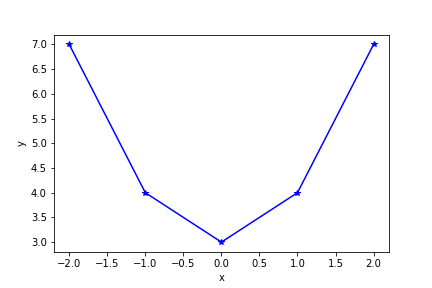
\includegraphics[width=8cm]{plot.png}
		\caption{Plot of y against x}
		\label{fig:data}
	\end{figure}
	In (a)(2), we realize that we could not attain a training loss of zero. To investigate this, we plot the data in Figure \ref{fig:data}. It seems like the $y$ is a quadratic function of $x$, instead of a linear function of $x$. Does it mean that we have no hope in getting a good linear regression model? The answer is no. We just need to be a little smart about our feature mapping $\phi$. Now, let us define a new feature mapping $\phi_2(x) = [1, x, x^2]$. With this new feature mapping, what is the closed form solution $\vec{w}$? Can we attain a training loss of zero with this closed form solution?
	
\end{enumerate}
\textbf{Take-away:} Feature extraction is essential in creating a powerful model. Although we will not cover how to design hand-crafted features, we will cover how to automatically learn a powerful representation of the data using kernel methods and possibly deep learning if time permits. 

\section*{Problem 3: Weighted Ridge Regression}
Suppose we have a dataset $\{(\vec{x}_1, y_1), ..., (\vec{x}_n, y_n)\}$. In a ridge regression setting, we assume that each example is equally important. Sometimes, certain examples are more important than others and we would want to assign a positive weight $p_i$ to each training examples to indicate the level of importance of each training example. For instance, in the previous problem, if we care more about the predictions of our model on the examples with positive $x$, then we might assign higher weights to those training examples with positive $x$ than those training examples with negative $x$. 
\newline
\newline
In order to modify ridge regression to account for the weights of different training examples, we rewrite the loss function as 
$$\ell(\vec{w}) = \sum_{i = 1}^{n}(p_i(\vec{w}^T\vec{x}_i - y_i)^2) + \lambda \vec{w}^T \vec{w}$$ where $\lambda \geq 0$.
\begin{enumerate}
	\item Suppose $X = [\vec{x}_1, ..., \vec{x}_n]^T$, $\vec{y} = [y_1, ..., y_n]^T$. Find a diagonal matrix P such that we can rewrite the loss function as $$\ell(\vec{w}) =  (X\vec{w} - \vec{y})^TP(X\vec{w} - \vec{y}) + \lambda \vec{w}^T \vec{w}$$
	\item Using the rewritten loss function, derive a closed form solution for $\vec{w}$ by setting the gradient of the loss function equal to zero. 
	\item Show that the loss function is convex by showing the $\nabla^2 \ell$ is positive semidefinite for any $\vec{w}$. By showing the loss function is convex, we can conclude that the closed formed we derived in (2) is indeed a global minimum point.  
\end{enumerate} 


\end{document}